\chapter{Preliminary Design}

This chapter aims to provide a general overview of the design, the interaction between the different modules of the NeoPixel Sunrise Clock (NPSC). Moreover, it provides the justifications of components selection and the reasoning behind the visual design of the NPSC.

%%%%%%%%%%%%%%%%%%%%%%%%%%%%%%%%%%%%%%%%%%%%%%%%%%%%%%%%%%%%%%%%%%%%%%%%%%%%%%%%%%%%
% SECTION: System overview
%%%%%%%%%%%%%%%%%%%%%%%%%%%%%%%%%%%%%%%%%%%%%%%%%%%%%%%%%%%%%%%%%%%%%%%%%%%%%%%%%%%%
\section{System overview}\label{system_overview}
The NPSC is designed such that it is a user-friendly bedside alarm-clock serving as a supplement in the treatment of sleep-disorder via light emission. To achieve these goals, the system was designed using a modular approach. The modules illustrated in  \cref{fig:strutural_block_diagram} are the elements deemed required to achieve the goals laid out in \ref{purpose_of_the_study}. \\
The relationship between the goals defined in the introduction and these modules are given below:
\begin{itemize}
\item \textbf{Regulate the sleep-wake cycle}: This is done by emissions of specific lights parameters using the Neopixel as part of the system outputs.
\item \textbf{User-friendly}: Using push-buttons for controlling the NPSC would not be optimal it is a multifunctional device. The onboard touchscreen in the System Inputs is to remove having the users relying on push-buttons to use certain functionalities. As for the android application, it allows the users to control the devices wirelessly. Via the Android application, the NPSC has the possibility to be an Internet Of Thing (IOT) device increasing the variety of its applications.
\item \textbf{Personalisable}: The system inputs are the doors to the NPSC configurations, with both inputs being touchscreen devices, multiples functionalities can be implemented. The EEPROM is to store user-specific data such as alarm, visual preferences.
\item \textbf{Alarm-clock}: The Clock module consisting of a Real Time Clock (RTC) and an Alarm are meant to interact together to make the NPSC also an alarm clock.
\end{itemize}
\begin{figure}[ht]
\centering
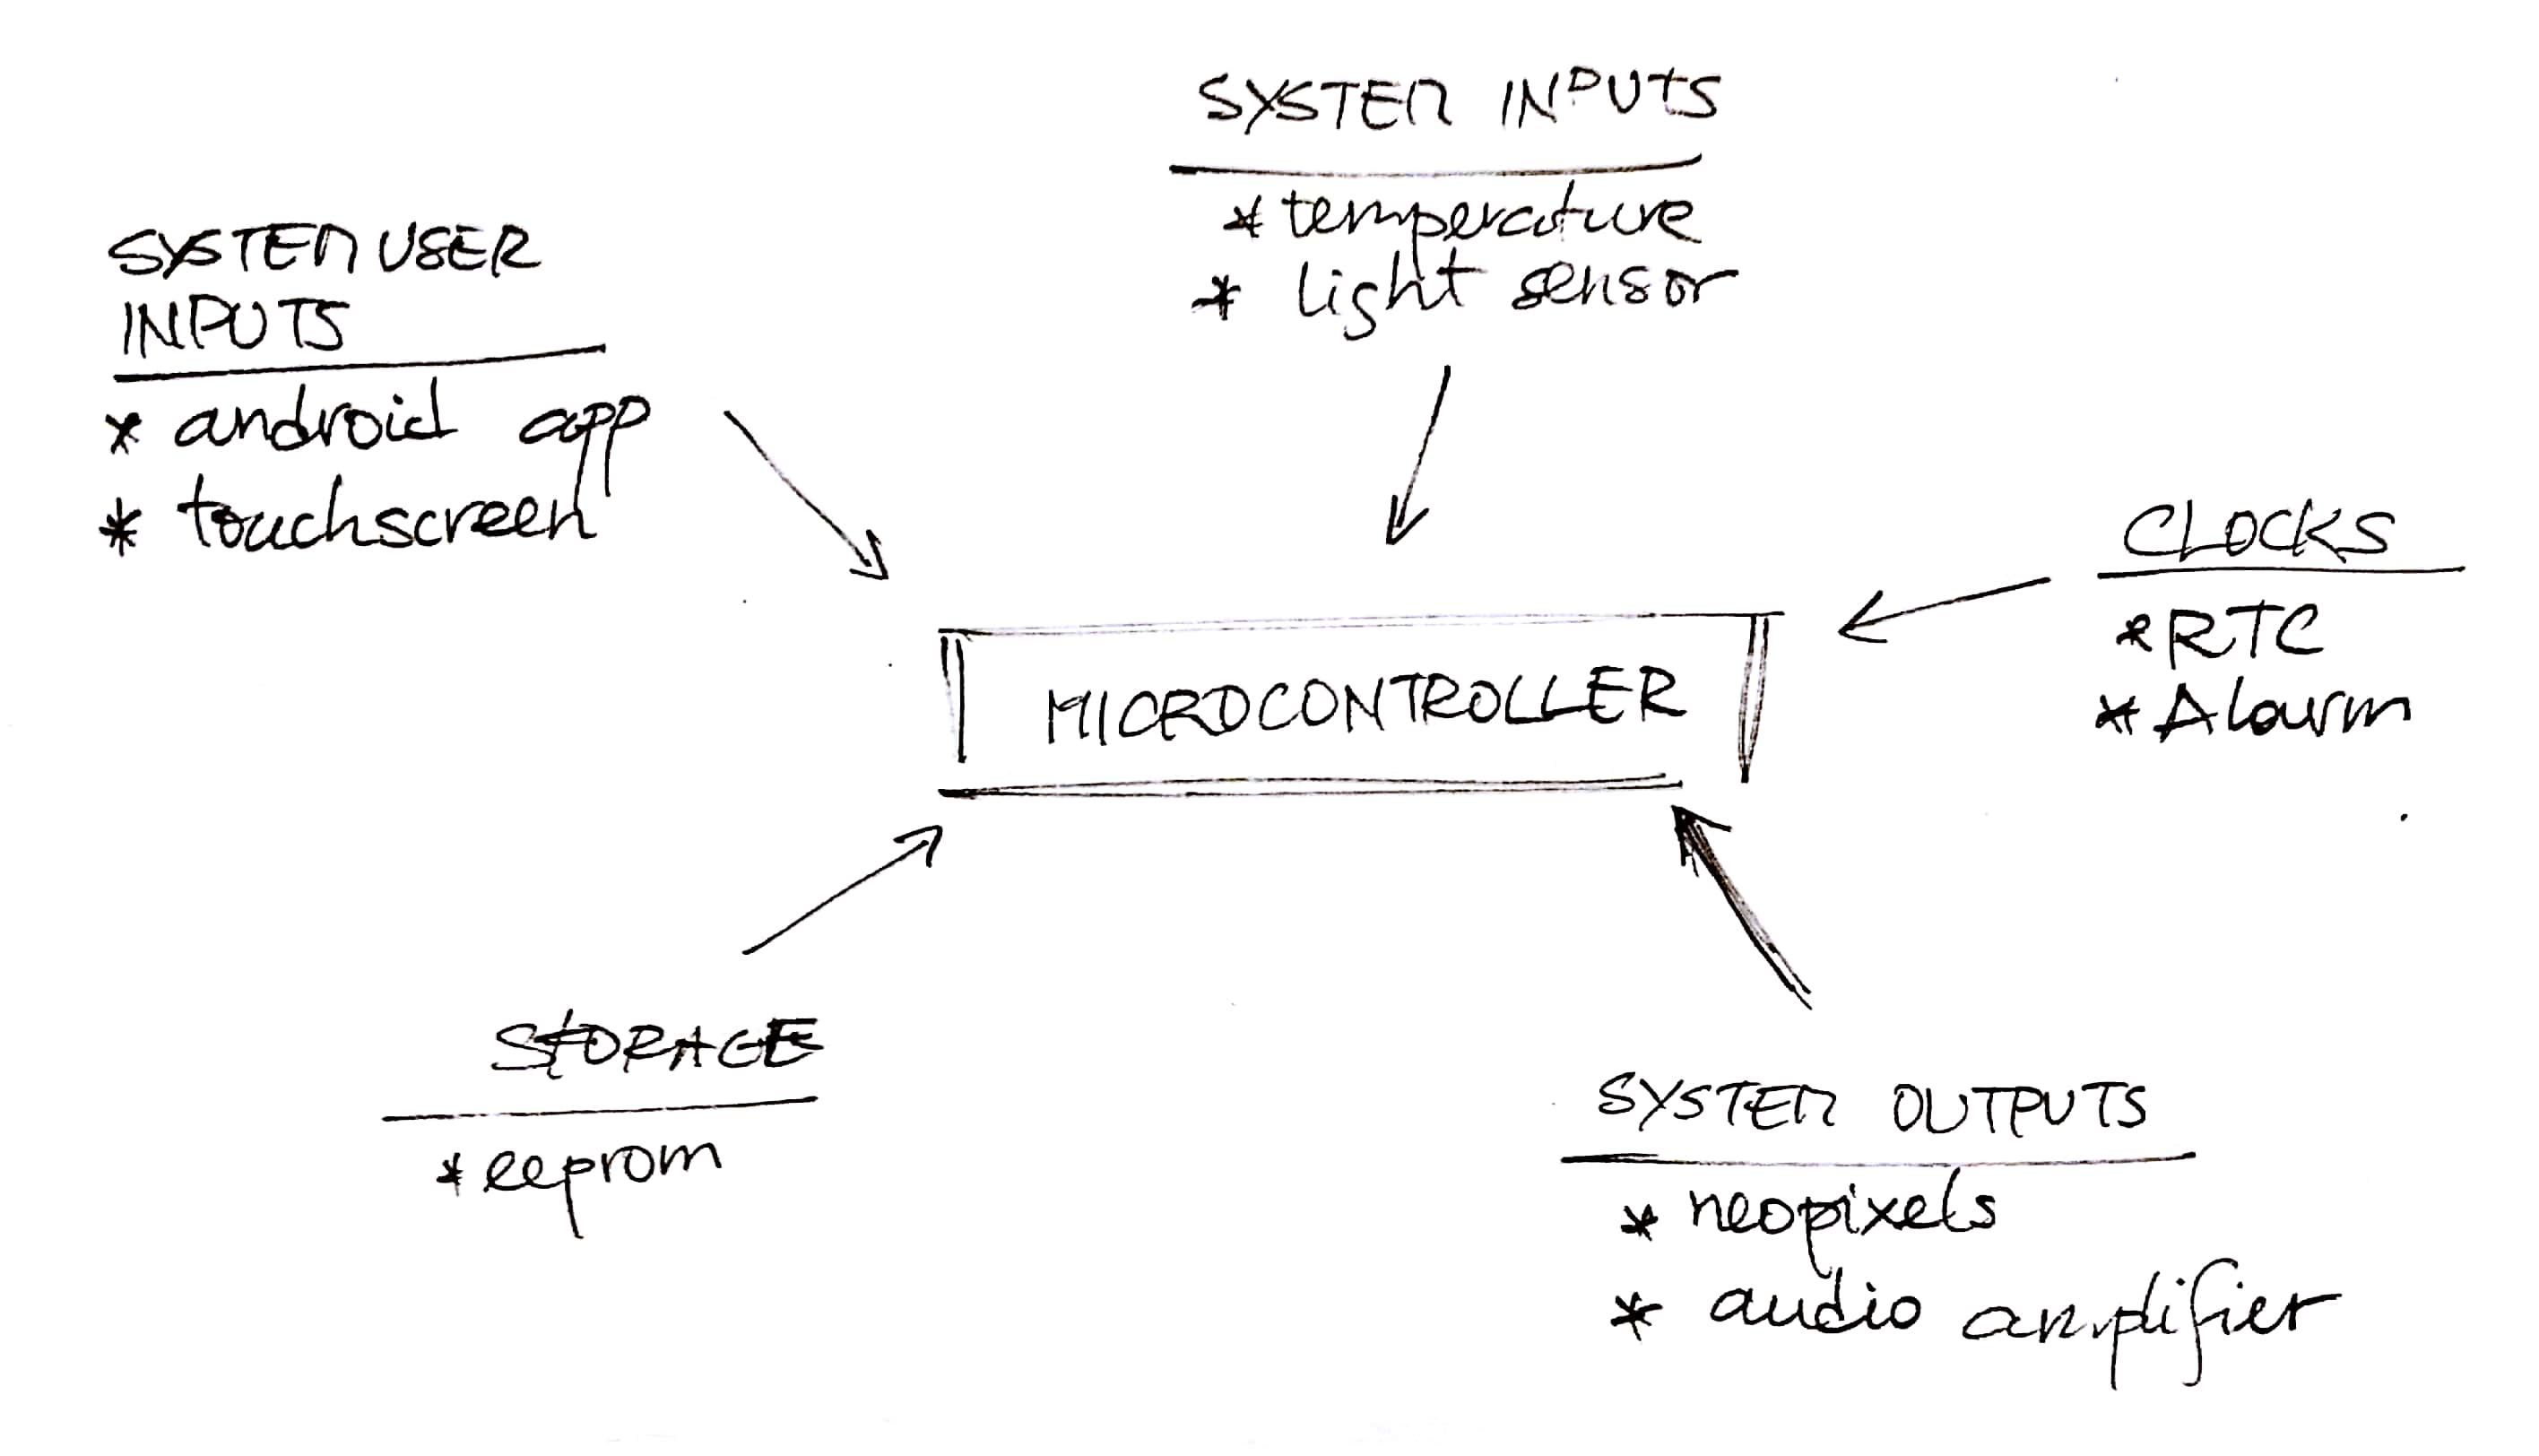
\includegraphics[scale=0.15]{strutural_block_diagram.jpg}
\caption{Structural block diagram of the NPSC.}
\label{fig:strutural_block_diagram}
\end{figure}


%%%%%%%%%%%%%%%%%%%%%%%%%%%%%%%%%%%%%%%%%%%%%%%%%%%%%%%%%%%%%%%%%%%%%%%%%%%%%%%%%%%%
% SECTION: System components selection 
%%%%%%%%%%%%%%%%%%%%%%%%%%%%%%%%%%%%%%%%%%%%%%%%%%%%%%%%%%%%%%%%%%%%%%%%%%%%%%%%%%%%
\section{System components selection}
This section provides reasons on the selection of the components described in \ref{system_overview}.  
\begin{itemize}
\item \textbf{Microcontroller}: The STM32F407VGT6 with the specifications listed in \cref{table:micro} is the one selected for the NPSC. This choice was based on its number of pins and mostly on the fact that this microcontroller has been used in previous projects. 
\item \textbf{Wireless}: As mentioned in \ref{wireless_technologies}, the preferable wireless technology is Bluetooth for its low complexity and the reliability of its connection. The HC-06 Bluetooth module has been chosen for this prototype for its popularity among microcontrollers application.
\item \textbf{Eeprom}: There are no specific requirements on the EEPROM selection, for this prototype, only few information might require to be stored. It was assumed that a 32KB EEPROM would be enough. The EEPROM chosen is the 25LC640 64KB as it was proven to be reliable in previous projects. Moreover, the framework for this EEPROM was already developed for an STM microcontroller in the third year Embedded System project.  
\item \textbf{RTC}: The NPSC is an alarm clock and must be able to get accurate time. The STM32F4 series have a built-in RTC with two alarms. Because this prototype might not run on batteries and the RTC data would be lost if the microcontroller loses power, an external RTC module was required. An off the shelves breakout board for an RTC (the DS1307) is heavily used as an RTC for microcontroller applications and is used for this project as the external RTC. This breakout board powers the DS1307 with a battery that can last 10 years.
\item \textbf{Light}: As mentioned in \ref{neopixels}, the Neopixels were used as light source.
\item \textbf{Touchscreen}: Many touchscreens on the market require the use of dozens of pins for their control. Besides, there are no common libraries for the modules increasing developing time. The touchscreen chosen for this prototype is the Nextion TFT touchscreen from Itead. It solves the issues mentioned above by providing an IDE (the Nextion IDE) used to program the screen via USB (required device from \ref{nextion}). It moreover provides an easy way for communicating with the microcontroller using two pins (TX and RX in the UART protocol).
\end{itemize}

%%%%%%%%%%%%%%%%%%%%%%%%%%%%%%%%%%%%%%%%%%%%%%%%%%%%%%%%%%%%%%%%%%%%%%%%%%%%%%%%%%%%
% SECTION: Visual outputs component design decision
%%%%%%%%%%%%%%%%%%%%%%%%%%%%%%%%%%%%%%%%%%%%%%%%%%%%%%%%%%%%%%%%%%%%%%%%%%%%%%%%%%%%
\section{Visual outputs component design decisions}
The NPSC's visual impact is very important as it has great influence on the users. While focusing on the visual impact, the NPSC light source must meet the light requirements. To achieve both aesthetic and functionalities, the preliminary aspects were considered:
\begin{itemize}
\item Light emission of $30lux$: This is an important function of the NPSC. To achieve this, the NPSC must have a main light source module, based on \cref{table:neopixel_illuminance}, 180 neopixels are sufficient to meet this requirement on a subject placed at $1m$ of the light source. For its aesthetic, the main light source is composed of three rings of 60 neopixels each. A great visual functionality could be displaying the hours, minutes and seconds one each ring, having the pixels on the seconds ring being light up as the second passes and so forth. Note that the board size needs to be large enough to dissipate the power consumed by the pixels (see \ref{PCB_requirement}).
\item Alarm clock: What is the purpose of the clock that does not display the time? For this reason - and to fill the gap in the centre of the ring - three main pieces of information are to be displayed:
\begin{enumerate}
\item Date and Temperature:  seven segments RGB displays are used to display this information. Using RGB displays provides consistency in the choice of colour that the NPSC can emit.
\item Time: A bigger version of the seven segments displays used in the point above could not be found, so the neopixels were used to simulate the seven segments RGB displays. 
\item Weekday: A row of seven neopixel, one for each day in the week.
\end{enumerate}
\end{itemize}

%%%%%%%%%%%%%%%%%%%%%%%%%%%%%%%%%%%%%%%%%%%%%%%%%%%%%%%%%%%%%%%%%%%%%%%%%%%%%%%%%%%%
% SECTION: Mechanical design
%%%%%%%%%%%%%%%%%%%%%%%%%%%%%%%%%%%%%%%%%%%%%%%%%%%%%%%%%%%%%%%%%%%%%%%%%%%%%%%%%%%%
\section{Mechanical case}
The NPSC must be able to stand on a bedside desk, these desks have a general size of $50cm*50cm$. The NPSC ideal mechanical design is displayed in \cref{fig:mechanical_prototype}.\\
Each side is meant to have specific use described below:
\begin{itemize}
\item \textbf{Front}: All visual outputs of the NPSC are on the front side. The main light source (the ring PCB) uses most of the front space. The other visual outputs PCBs are designed to fit inside the ring. The front side should be covered by a material hiding the PCB but letting most of the light pass. Here the NPSC should provide the look of a dark glass whose part can be illuminated.
\item \textbf{Top}: The onboard touchscreen is located on the top of the NPSC. The touchscreen should be detachable from the NPSC case to allow the user to view the changes on the board while modifications are made.
\item \textbf{Right and Left side}: Each side should have a speaker for the alarm. On the right side on the NPSC, a set of critical buttons are used to power off the device or stop the alarm.
\end{itemize} 
\begin{figure}[ht]
\centering
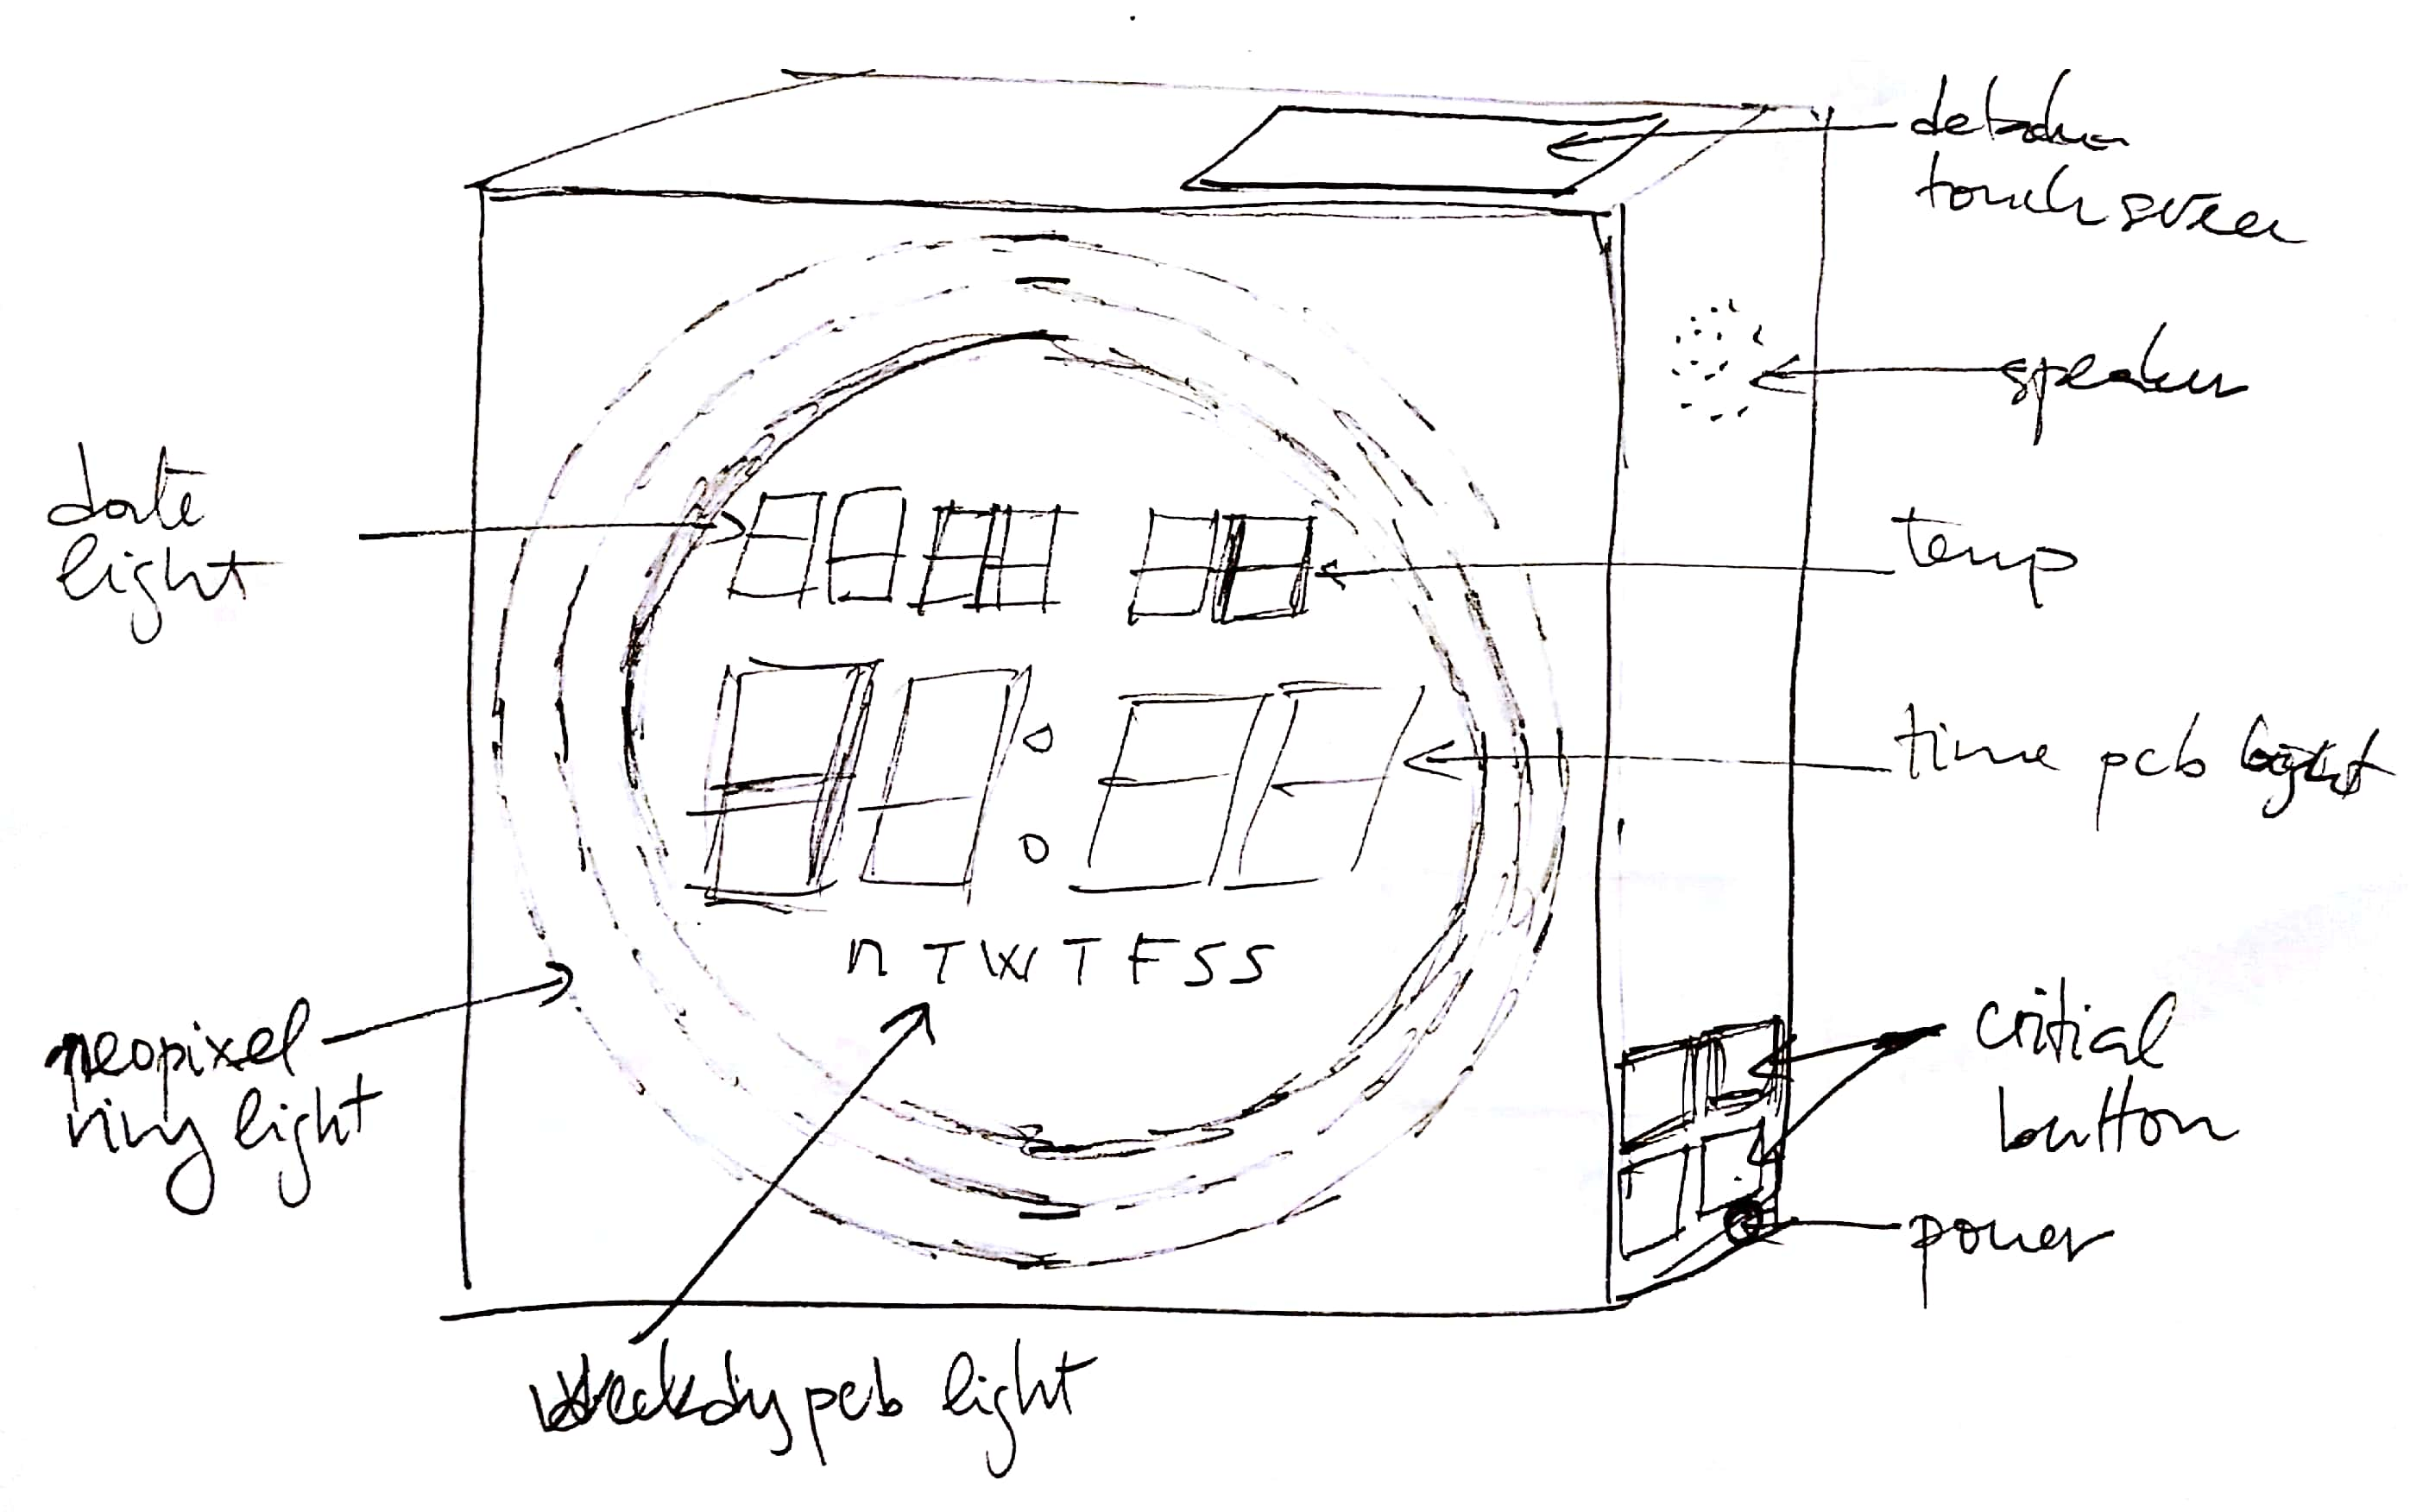
\includegraphics[scale=0.15]{mechanical_prototype.jpg}
\caption{Mechanical prototype of the NPSC.}
\label{fig:mechanical_prototype}
\end{figure}